\chapter{Stopwatch Control Unit}
\label{chapter:stopControl}
\graphicspath{ {./Lab10ControlUnit/Fig} }

\section{Outcomes and Objectives}

The outcome of this lab is to design and simulate
a control unit to control the datapath that stores and
manipulates the information need to run a stopwatch.
Through this process you will achieve the following
learning objectives.
\begin{itemize}
    \item \Paste{bok:FSM_Timing}
    \item \Paste{bok:DaC_ControWord}
    \item \Paste{HDL:Do}
    \item \Paste{VER:fsm}
\end{itemize}

\section{Stopwatch}

From the previous lab, you should be familiar with the operation of our
stopwatch. Briefly, our stopwatch allows a user to measure elapsed time
and lap times of a competitive events. Our stopwatch measures time in
increments of a tenth of a second, unit second and tens of seconds.
Control input comes from 2 buttons called S1 and S2 according to the
incomplete finite state machine shown in Figure~\ref{fig:swCuHighLevel}.

\begin{figure}[ht]
    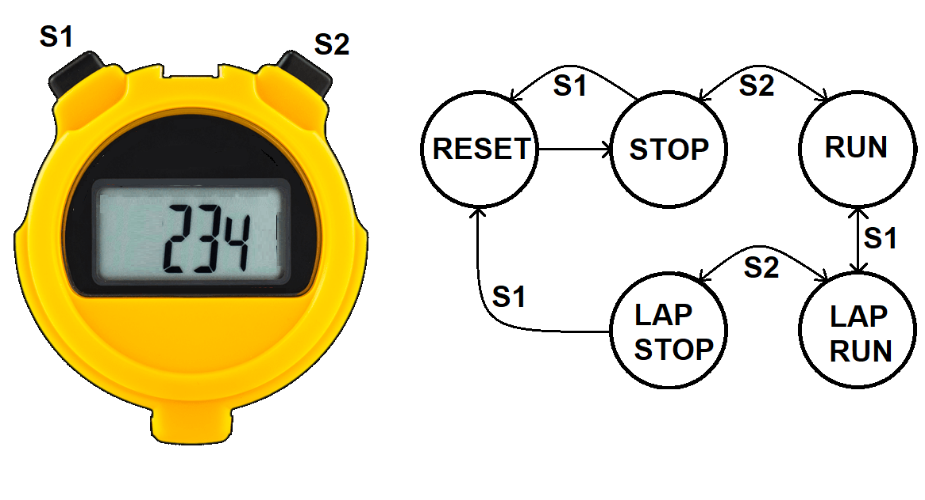
\includegraphics[width=0.4\paperwidth]{image1.png}
    \caption{ A digital stopwatch gets its input from 2 buttons and displays
        its output on a 7-segment display. The behavior of the stopwatch can be
    described by this finite state machine (FSM).}
    \label{fig:swCuHighLevel}
\end{figure}

There are two reasons that the FSM shown in in Figure~\ref{fig:swCuHighLevel} is incomplete,
it does not reflect the logic level of the buttons on the FPGA development board nor
does it account for the time the user holds the S1 and S2 buttons down.

Figure~\ref{fig:swCuButtons} shows the schematic of the buttons (key1 \ldots key4) on the
C5G development board that you will use to control the operation of the
stopwatch; the S1 and S2 buttons in Figure~\ref{fig:swCuHighLevel}. The buttons shown in the
schematic are in their nominal position -- not being pressed by a user.
You should note that the contacts of each button (open circles) are
disconnected. This leaves the right side of the button connected to VCC
through a resistor as well as the Altera FPGA. This resistor is called a
pull-up resistor, and as its name implies, pulls the voltage on the
right side of the push button up to VCC -- logic 1. When a button is
pressed, the contacts are connected and the right side of the push
button is connected directly to ground, forcing the voltage on the
respective FPGA pin to logic 0.

\begin{figure}[ht]
    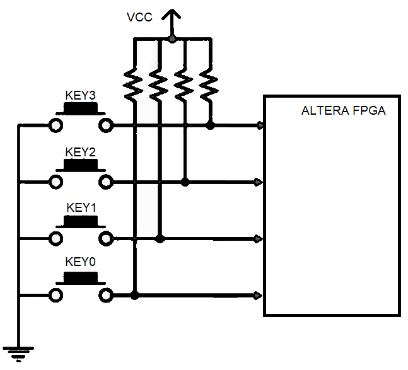
\includegraphics[width=0.4\paperwidth]{image2.png}
    \caption{FPGA development board buttons used to operate the stopwatch.}
    \label{fig:swCuButtons}
\end{figure}

To summarize the operation of the buttons shown in Figure~\ref{fig:swCuButtons}. When a user
presses a button, the value on the respective FPGA pin is logic 0. When
a button is not pressed, the logic level of the corresponding FPGA pin
is logic 1.

You will explore the reason that effect of the user holding down a
button in the next section which introduces you to the finite state
machine that governs the behavior of your stopwatch.

\section{Module: \hdl{stopWatchControl}}
The design of the stopwatch controller starts with the state diagram, then
on to the control word values for each state, and then finally to the
Verilog code needed to implement the state diagram and control
word.  Each of these steps is outlined below.

\subsection{State diagram for stopWatchControl}
The state diagram for the stopwatch is shown in Figure~\ref{fig:swCuStateDiagram}.
\begin{figure}[ht]
    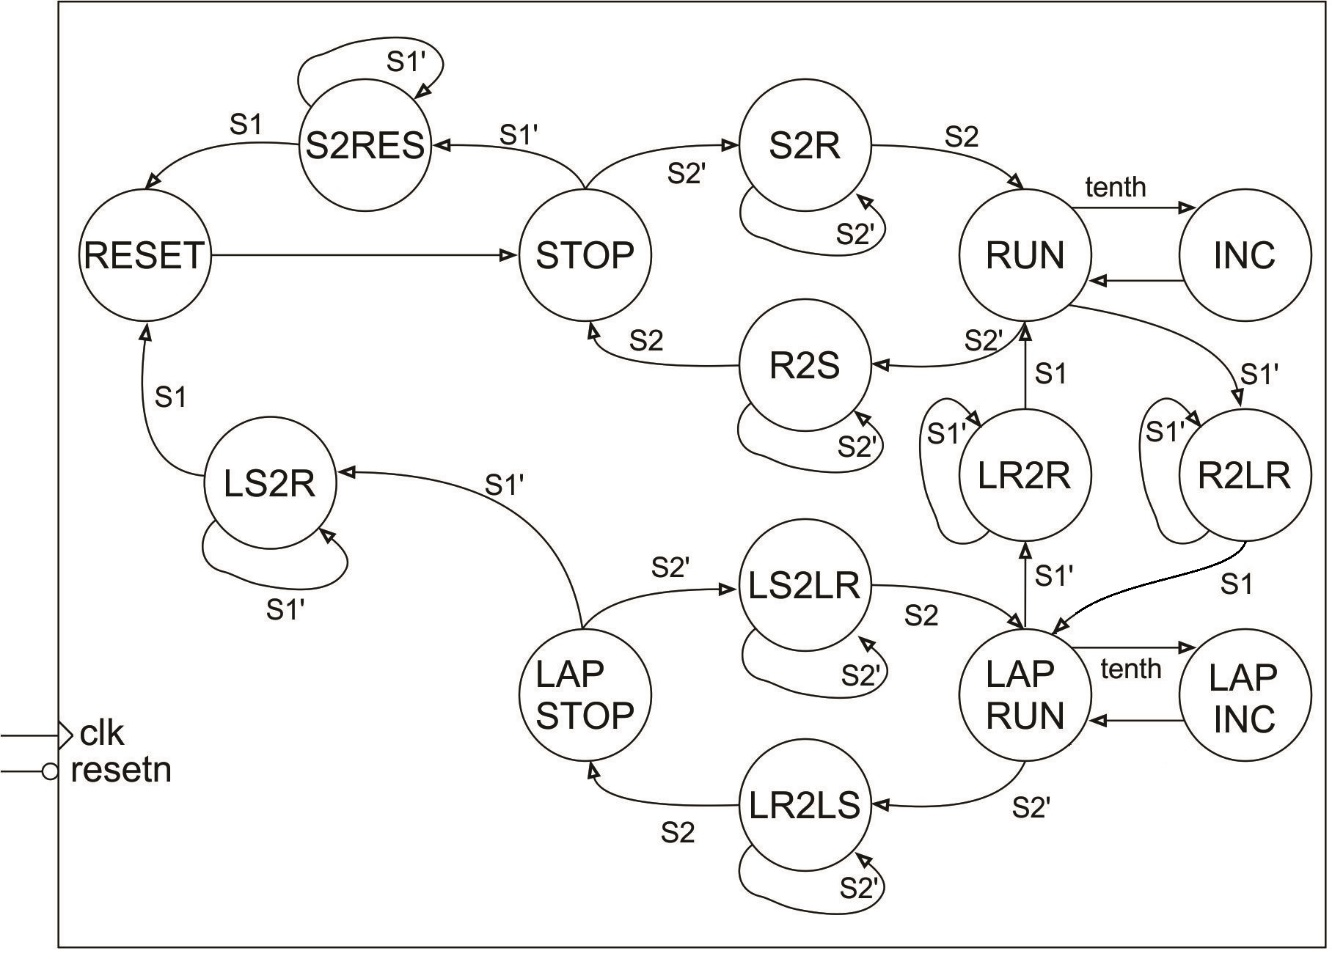
\includegraphics{image3.jpeg}
    \caption{The control unit for the stopwatch needs to account for the
    time the user holds the button down.}
    \label{fig:swCuStateDiagram}
\end{figure}
The arcs between states are labeled with a Boolean condition, which when
true, causes the FSM to make that transition. So for example, if the FSM
is in the RUN state and the S2 button is pressed (buttons output 0 when
pressed hence the arc labeled S2'), the FSM will transition to the R2S
state (and stay there as long as the button is held down). When a number
``2'' appears in the middle of a state name, the number denotes the word
``to'' which is intended to mean moving from one state to another. The
abbreviated names of the source/destination states are written on
left/right side of the number ``2'' respectively. So for example, the
state R2S stands for Run to Stop.

These intermediate states are needed because the action of a user
pressing a button takes a long time from the perspective of the 50MHz
clock on the FPGA development board. For example, consider the incorrectly designed FSM
shown in Figure~\ref{fig:swCuImproperFsm}. The intention of this design is to have the FSM
transition from the STOP state to the RUN state when the user pressed
the button S2 (remember that when S2 is pressed it outputs a logic 0,
hence the arc labeled S2'). What actually happens is that the FSM
rapidly toggles between the STOP and RUN states at 50MHz while the S2
button is held down. When the user releases the S2 button there is a
50/50 chance that the FSM will end-up in the STOP or RUN state.

\begin{figure}[ht]
    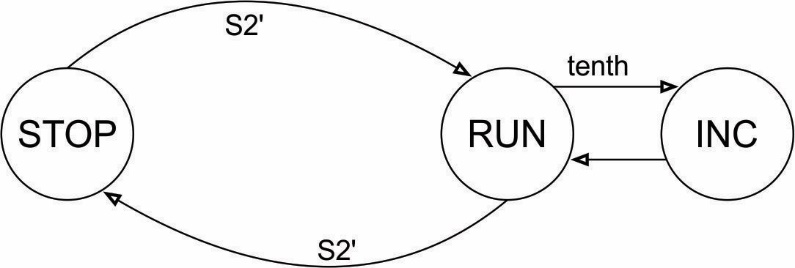
\includegraphics{image4.jpeg}
    \caption{An improperly constructed FSM for the stopwatch.}
    \label{fig:swCuImproperFsm}
\end{figure}

\subsection{Control word for stopWatchControl}
Before you dive into writing the Verilog code for the control unit, you
need to complete Table~\ref{table:swCuControlWord}, the control word value for each state. You
have already completed some of these control words in the previous lab.
Most of the new states are the states with ``2'' in them. We will call
these ``transitional states'' because they move the control unit between
stopwatch modes. When writing the control words in Table~\ref{table:swCuControlWord} you must
follow the following 2 rules.

\begin{enumerate}
    \def\labelenumi{\arabic{enumi})}
\item
    Assign the cw{[}5{]} bit for transitional states the same value as the
    cw{[}5{]} value for the source state. So for example in the R2LR
    state, set cw{[}5{]} to 0 because the cw{[}5{]} value in the source
    state, RUN, is 0.
\item
    Only have the timer counter counting up while the control unit is in
    the RUN or LAPRUN states. We don't want the timer counting up in
    intermediate states because these states do not have an ``INC''
    associated with them, and as a consequence, the tenth pulse from the
    timer counter would most likely be missed.
\end{enumerate}

\begin{longtable}[]{@{}
    | >{\raggedright\arraybackslash}p{(\columnwidth - 10\tabcolsep) * \real{0.1666}}|
    >{\raggedright\arraybackslash}p{(\columnwidth - 10\tabcolsep) * \real{0.1666}}|
    >{\raggedright\arraybackslash}p{(\columnwidth - 10\tabcolsep) * \real{0.1666}}|
    >{\raggedright\arraybackslash}p{(\columnwidth - 10\tabcolsep) * \real{0.1666}}|
    >{\raggedright\arraybackslash}p{(\columnwidth - 10\tabcolsep) * \real{0.1667}}|
>{\raggedright\arraybackslash}p{(\columnwidth - 10\tabcolsep) * \real{0.1667}}|@{}}
\caption{Control word table for the stopwatch finite state
machine shown in Figure~\ref{fig:swCuStateDiagram}.}\label{table:swCuControlWord}\tabularnewline
\toprule()
\begin{minipage}[b]{\linewidth}\raggedright
\end{minipage} &
\begin{minipage}[b]{\linewidth}\raggedright
    cw{[}5{]}

    2x1 mux
\end{minipage} &
\begin{minipage}[b]{\linewidth}\raggedright
    cw{[}4{]}

    lap register
\end{minipage} &
\begin{minipage}[b]{\linewidth}\raggedright
    cw{[}3{]}

    mod 10 reset
\end{minipage} &
\begin{minipage}[b]{\linewidth}\raggedright
    cw{[}2{]}

    mod10 count
\end{minipage} &
\begin{minipage}[b]{\linewidth}\raggedright
    cw{[}1:0{]}

    timer counter
\end{minipage} \\
\midrule()
\endfirsthead
\toprule()
\begin{minipage}[b]{\linewidth}\raggedright
\end{minipage} &
\begin{minipage}[b]{\linewidth}\raggedright
    cw{[}5{]}

    2x1 mux
\end{minipage} &
\begin{minipage}[b]{\linewidth}\raggedright
    cw{[}4{]}

    lap register
\end{minipage} &
\begin{minipage}[b]{\linewidth}\raggedright
    cw{[}3{]}

    mod 10 reset
\end{minipage} &
\begin{minipage}[b]{\linewidth}\raggedright
    cw{[}2{]}

    mod10 count
\end{minipage} &
\begin{minipage}[b]{\linewidth}\raggedright
    cw{[}1:0{]}

    timer counter
\end{minipage} \\
\midrule()
\endhead
& 0 = mod10 & 1 = load & 1 = reset & 1 = count up & 11 = load \\ \hline
& 1 = register & 0 = hold & 0 = hold & 0 = hold & 10 = count up \\ \hline
& & & & & 01 = not used \\ \hline
& & & & & 00 = hold \\ \hline
RESET & & & & 0 & \\ \hline
STOP & & & & & \\ \hline
S2RES & & & & & \\ \hline
S2R & & & & & \\ \hline
RUN & 0 & & & & \\ \hline
R2LR & 0 & & & & \\ \hline
R2S & & & & & \\ \hline
INC & & & & & \\ \hline
LAPRUN & & & & & 10 \\ \hline
LR2R & & & & & \\ \hline
LR2LS & & & & & \\ \hline
LAPINC & & & & & \\ \hline
LAPSTOP & & & 0 & & \\ \hline
LS2R & & & & & \\ \hline
LS2LR & & & & & \\
\bottomrule()
\end{longtable}

\subsection{Verilog code for stopWatchControl}
\label{subsubsection:swCuVerilog}
After you complete the control word table, you are ready to write the
Verilog for the control unit. This file will have the following main
sections.

\begin{itemize}
\item
    Port description -- This has been provided to you.
\item
    Control word values -- This is a set of localparam statements, one for
    each state. You will define the control word output for each state.
    This will include all the control words that you derived in the
    previous lab, plus some new control words for the intermediate states.
    For example, the following is the control word for the STOP state.
\end{itemize}

\hdl{localparam STOP\_CW = 6'b000000;}

\begin{itemize}
\item
    State codes -- Each state needs to be assigned a unique binary value.
    It does not matter what code you assign which state. These codes are
    mostly invisible. That said, you will want them handy when performing
    the simulation so that you know which state the control unit is in.
    For example, the following is the state code that I used for the STOP
    state. Note, your codes can be different.
\end{itemize}

\hdl{TOP\_STATE = 4'b0010,}

\begin{itemize}
\item
    Reset logic -- this has been provided to you.
\item
    Output logic -- This is an always/case statement that has one case for
    each state and simple associated the control word output with the
    appropriate control word for the state that the FSM is currently in.
    For example, the following is the case statement that I used to
    associate the STOP state control word with the STOP state code.
\end{itemize}

\hdl{STOP\_STATE: cw = STOP\_CW;}

\begin{itemize}
\item
    Next state logic -- This is an always/case statement that has one case
    for each state. It embodies the logic in Figure~\ref{fig:swCuStateDiagram} using if/then
    statements. Let's redraw Figure~\ref{fig:swCuStateDiagram} by focusing on the states connected
    to the STOP state by transition arcs in Figure~\ref{fig:swCuStopState}.
\end{itemize}

\begin{figure}[ht]
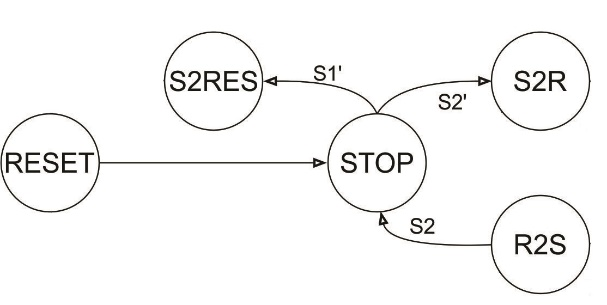
\includegraphics{image5.jpeg}
\caption{All the states and with a transition arc connected to the STOP state.}
\label{fig:swCuStopState}
\end{figure}

The next state logic for the STOP state embodies the 2 transition arcs
leaving the STOP state in Figure~\ref{fig:swCuStopState}. If the FSM is in the STOP state and
the S1 input equals 1 then the FSM should go to the S2RES state. This
logic and the transition to the state S2R is provided in the following
code snippet. You must specify every possible next state, even when the
next state does not change. Thus, I prefer to use a case statement and
leave the default case to be when the next state is equal to the current
state.

\begin{lstlisting}[language=Verilog,  frame=single]
    STOP_STATE:
        begin
            case({S2,S1})
                2'b10: nextstate = S2RES_STATE;
                2'b01: nextstate = S2R_STATE;
                default: nextstate = STOP_STATE;
            endcase
        end
\end{lstlisting}

When writing code for the control unit, I want you to:

\begin{itemize}
\item
    Use the controlUnit.v file provided in the Canvas folder as the
    starting point.
\item
    Provide meaningful names to the wires in the module.
\item
    Properly tab-indent your code. You can use View -\textgreater{} Show
    White Space

    \begin{itemize}
        \item
            Single level for wire declarations
        \item
            Single level for component instantiations
        \item
            Two levels for case statement
        \item
            Three levels for case values
    \end{itemize}
\end{itemize}

Compile the Verilog code for the control unit, look for and remove the
errors. When the control unit compiles cleanly, it's time to simulate to
check that it behaves correctly.

\section{Testbench}
This lab will terminate with an extensive simulation of the stopwatch to
uncover as many bugs as
possible. Errors are much, much easier to find in a
simulation. The goal of this simulation is to cover every transition arc
in Figure~\ref{fig:swCuStateDiagram} so that you can be sure your code is working correct.

The timing diagrams shown in Figure~\ref{fig:swCuSimTiming} show the tenths,
S1 and S2 signals as they are manipulated by the testbench. These
signals will affect the state of the control unit according to Figure~\ref{fig:swCuStateDiagram}.
Your task is to use these signals to determine what the state the
control unit is in.

The goal of the testbench was to cover every transition arc in Figure~\ref{fig:swCuStateDiagram}.
This goal was not achieved; one transition arc was not taken in the
testbench, which one was it?

\begin{landscape}

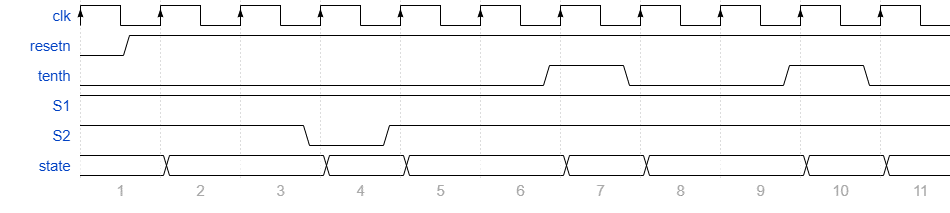
\includegraphics{image7.png}

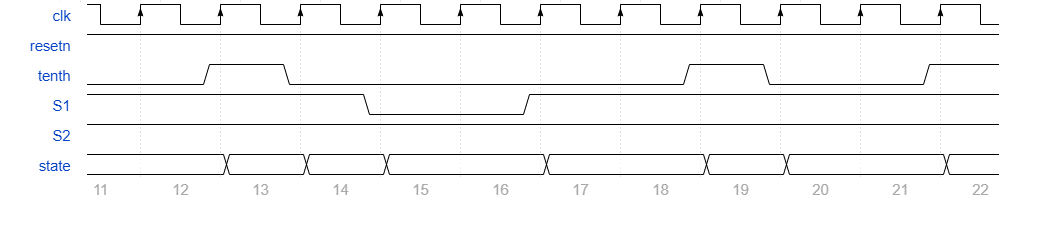
\includegraphics{image8.png}

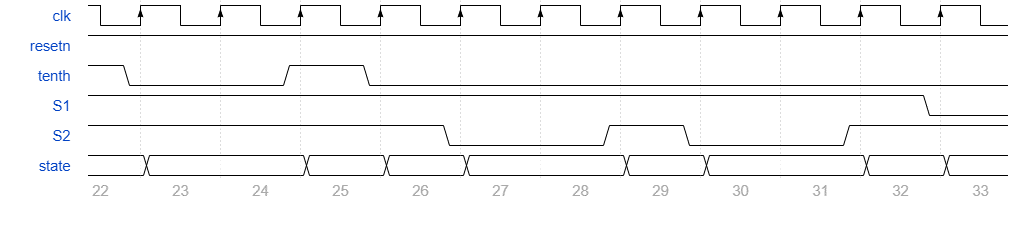
\includegraphics{image9.png}

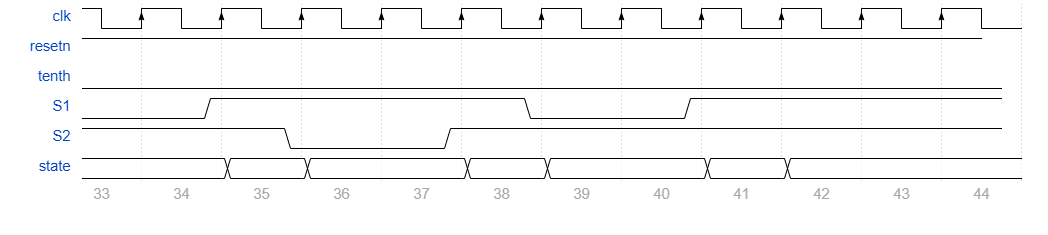
\includegraphics{image10.png}
\begin{figure}
    \caption{Timing diagram for the testbench for the testbench simulation}.
    \label{fig:swCuSimTiming}
\end{figure}
\end{landscape}

Now that you have an understanding of what the testbench should do, it's
time to run the simulation. Complete the provided do file to simplify
testing your control unit. Your timing diagram should have the following
\hypertarget{swCuWaveform}{%
waveforms.
\label{swCuWaveform}}

\begin{tabular}{p{0.5cm}p{1.5cm}p{5cm}p{3cm}}
signal & radix & trace color \\ \hline
clk         & & default         & green trace    \\
resetn     & & default         & green trace    \\
cw         & & hex         & yellow trace    \\
tenth     & & default         & orange trace    \\
S2         & & default         & orange trace    \\
S1         & & default         & orange trace    \\
states     & &           &            \\
& stop/stop2reset/reset/stop2run             & & red trace    \\
& run/inc/run2lapRun/run2stop             & & yellow     trace\\
& lapRun/lapInc/lapRun2run/lapRun2lapStop    & & orange  trace\\
& lapStop/lapStop2run/lapStop2LapRun           &  & green  trace\\
\end{tabular}\\

When editing the do file for this lab, note the following.

\begin{itemize}
\item
    Correct the waveform names as needed. This might happen if you name a
    signal differently than I did.
\item
    Create alias' for each state code. When you coded the control unit by
    assigning an arbitrary 4-bit value to each state. In Listing~\ref{listing:swCuDoFileState} you
    will associate each of these 4-bit values to a string and a color. The
    string should correspond to the name of the state and the color to
    something identifiable when the simulation is running. For example,
    you may remember that I assigned STOP\_STATE =
    4\textquotesingle b0010. This corresponds to the line
    ``4\textquotesingle b0010 "STOP" -color red,'' in Listing~\ref{listing:swCuDoFileState}

  \begin{lstlisting}[language=Verilog,
 caption={Creating alias' for the binary codes of states in the do file uses requires knowing the binary code of each state, the name of each state and the color for each state.},
 label={listing:swCuDoFileState},
 frame=single]
 radix define States {
        ...
    4'b0010 "STOP"    -color red,
        ...
    -default hex
    -defaultcolor white
}
 \end{lstlisting}

\item
    This will produce a much more meaningful representation like that
    shown in Figure~\ref{fig:swCuTestbenchTiming} of the state when you run the simulation.
\end{itemize}

\begin{figure}[ht]
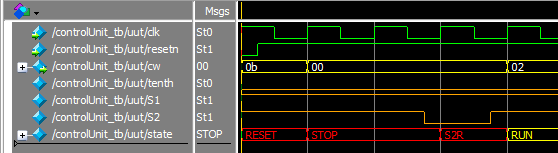
\includegraphics[width=0.6\paperwidth]{image11.png}
\caption{A small segment of the testbench simulation showing how
Listing~\ref{listing:swCuDoFileState} encodes state names.}
\label{fig:swCuTestbenchTiming}
\end{figure}

Run the entire simulation and compare the simulation output to Figure~\ref{fig:swCuSimTiming}.
Use the results of the simulation to either correct Figure~\ref{fig:swCuSimTiming} or
to correct your controlUnit.v code.

\section{Turn in}

You may work in teams of at most two. Make a record of your response to
the items below and turn them in a single copy as your team's solution
on Canvas using the instructions posted there. Include the names of both
team members at the top of your solutions. Use complete English
sentences to introduce what each of the following listed items (below)
is and how it was derived. In addition to this submission, you will be
expected to demonstrate your circuit at the beginning of your lab
section next week.

\subsubsection{Control Unit Design}

\begin{itemize}
\item
    Completed Table~\ref{table:swCuControlWord}.
\item
    Completed Figure~\ref{fig:swCuSimTiming}.
\item
    Verilog code for the control unit in Section~\ref{subsubsection:swCuVerilog}.  Only
    include Verilog code for the body of the control unit module (courier 8-point
    font single spaced) - leave out header comments.
\end{itemize}

\subsubsection{Control Unit Simulation}

\begin{itemize}
\item
    Timing diagram of control unit \hyperlink{swCuWaveform}{simulation} .
\end{itemize}

\begin{itemize}
\item
    Demonstrate your simulation to a member of the lab team.
\end{itemize}
